\documentclass[conference]{IEEEtran}
\usepackage[utf8]{inputenc}
\usepackage[T1]{fontenc}
\usepackage{amsmath,amssymb}
\usepackage{graphicx}
\usepackage{booktabs}
\usepackage{multirow}
\usepackage{array}
\usepackage{xcolor}
\usepackage{cite}
\usepackage{url}
\usepackage[hidelinks]{hyperref}
\usepackage{tikz}
\usetikzlibrary{positioning,arrows.meta,shapes.geometric,fit,calc}

% If main.tex is in the repo root, change to \newcommand{\figdir}{report_figures/}
\newcommand{\figdir}{../report_figures/}
\newcommand{\safegraphic}[2][width=\linewidth]{%
  \IfFileExists{\figdir#2}{\includegraphics[#1]{\figdir#2}}{%
  \fbox{\parbox{0.85\linewidth}{\centering\footnotesize Missing figure:\\ \detokenize{#2}}}}}
\newcommand{\todo}[1]{\textcolor{red}{[TODO: #1]}}
\newcommand{\ssim}{\mathrm{SSIM}}
\newcommand{\lone}{\mathcal{L}_1}

\begin{document}

\title{Universal, Hard-Routed and Soft Mixture-of-Experts Image Restoration and Style-Conditioned Face-to-Sketch Generation: From Research to a Containerised Application}

\author{\IEEEauthorblockN{\todo{Maryam Fatima}}
\IEEEauthorblockA{\todo{23i-0788}, \todo{Computer Science}, FAST-NUCES\\
Email: \todo{email}\\
Code: \url{https://github.com/Maryam-Faatima/genai-restoration-sketch-studio}\\
Demo video: \todo{YouTube link}}}

\maketitle

\begin{abstract}
We build and evaluate four related generative systems and deploy them in one browser-based application. On the Oxford-IIIT Pet dataset we study image restoration under three runtime corruptions (salt-and-pepper noise, Gaussian blur, rectangular occlusion): (i) a universal convolutional autoencoder with a genuine bottleneck, (ii) a hard-routed system in which a corruption classifier selects one of three specialist autoencoders, and (iii) a jointly fine-tuned soft mixture-of-experts (MoE) with a differentiable gate and an identity branch. On the FS2K dataset we train (iv) a style-conditioned U-Net/PatchGAN face-to-sketch generator. On a fixed test manifest of 36{,}690 corrupted images the classifier reaches 99.8\% accuracy, hard routing reaches 26.56\,dB PSNR / 0.804 SSIM and soft MoE reaches 26.91\,dB / 0.828 against 22.34\,dB / 0.671 for the unrestored inputs (the overall averages include clean images). The face-to-sketch generator reaches 0.486 SSIM on the official test set and produces visibly blurry sketches, which we analyse. All hyperparameters were tuned with Optuna, experiments were tracked with Weights \& Biases, all inference models were exported to ONNX and verified against PyTorch (maximum absolute difference $1.3\times10^{-6}$), and everything is served through a FastAPI backend and a React frontend started with a single Docker Compose command.
\end{abstract}

\begin{IEEEkeywords}
denoising autoencoder, mixture of experts, image restoration, conditional GAN, Optuna, ONNX, FastAPI
\end{IEEEkeywords}

%=====================================================================
\section{Introduction}
Real-world images are rarely degraded in one known way. A restoration system must therefore either handle every corruption with one model, decide which specialist to apply, or blend specialists. This work compares these three designs under identical data, splits and metrics, and adds a paired image-to-image generation task. We also treat the project as a software product: every model is exported to ONNX and reachable through one web application.

Our contributions are: (1) a reproducible runtime-corruption pipeline with deterministic validation and test manifests; (2) a documented design history of the universal autoencoder (v1--v3) with controlled ablations; (3) a hard-routed system evaluated with both oracle and predicted routing; (4) a soft MoE initialised from the hard-routed components, with an analysis of its gate; (5) a style-conditioned cGAN with a style embedding used in both generator and discriminator; and (6) a containerised application whose models match their PyTorch originals.

%=====================================================================
\section{Related Work}
\textbf{Restoration with autoencoders.} Denoising autoencoders learn to reconstruct clean inputs from corrupted ones \cite{vincent2008}; convolutional denoisers such as DnCNN \cite{zhang2017dncnn} and inpainting networks \cite{pathak2016} extend this to images. Skip connections as in U-Net \cite{ronneberger2015} preserve detail but, when unrestricted, let a network copy its input, which defeats a compression bottleneck. Combining an $L_1$ term with a structural-similarity term is a well-studied loss for restoration \cite{zhao2017loss,wang2004ssim}.

\textbf{Mixtures of experts.} Mixtures of experts combine specialists through a gating network \cite{jacobs1991}. Sparse gating at scale \cite{shazeer2017} and later work \cite{fedus2022} motivate auxiliary losses that keep expert usage balanced; we use a differentiable balance term for the same reason.

\textbf{Conditional generation.} GANs \cite{goodfellow2014} and their conditional form \cite{mirza2014} underlie paired translation with a U-Net generator and PatchGAN discriminator \cite{isola2017}. Feature-wise linear modulation (FiLM) \cite{perez2018} injects a condition into intermediate features, which we use for the style embedding. FS2K \cite{fan2022fs2k} provides photo--sketch pairs in three styles.

\textbf{Tooling.} Hyperparameters were optimised with Optuna \cite{akiba2019}, experiments tracked with Weights \& Biases \cite{biewald2020}, and models served with ONNX Runtime \cite{onnxrt}.

%=====================================================================
\section{Datasets and Experimental Setup}
\subsection{Oxford-IIIT Pet (Tasks 1--3)}
We use the Oxford-IIIT Pet dataset \cite{parkhi2012}. Images are converted to RGB and resized to $128\times128$. The official \texttt{trainval} collection (3{,}680 images) is split 80/20 with random seed 42 into 2{,}944 training and 736 validation images (no overlap). The official test set (3{,}669 images) was held out. Class labels are unused: the clean image is the target. The same split is used for Tasks 1--3.

\subsection{Runtime corruptions}
During training the data loader draws, with equal probability, one of four input conditions for every loaded image and samples fresh parameters from operating-system entropy, so no corrupted copies are stored. Table~\ref{tab:corr} gives the definitions. The condition label is returned with each sample and trains the classifier of Task 2. Training batches for the classifier and the soft MoE are exactly balanced (verified: \texttt{[8, 8, 8, 8]} per batch of 32).

\begin{table}[t]
\centering
\caption{Corruption definitions. Test severities are fixed.}\label{tab:corr}
\footnotesize\setlength{\tabcolsep}{3pt}
\begin{tabular}{@{}p{1.6cm}p{2.7cm}p{2.5cm}@{}}
\toprule
Condition & Training (random) & Test (low/med/high)\\
\midrule
Clean & none & none\\
Salt-and-pepper & $p\sim U(0.02,0.15)$, black/white equally likely & $p=0.03,\,0.08,\,0.15$\\
Gaussian blur & kernel $\in\{3,5,7\}$, $\sigma\sim U(0.5,2.5)$ & $(3,0.7),(5,1.5),(7,2.5)$\\
Occlusion & 1--3 black rectangles, joint area 10--35\% & 1, 2, 3 rectangles covering $\approx$10, 20, 35\%\\
\bottomrule
\end{tabular}
\end{table}

\subsection{Deterministic manifests}
Validation and test corruptions are generated once and stored in JSON manifests (type, severity, blur settings, rectangle coordinates and seed per entry). The validation manifest has 736 entries (exactly 184 per condition). The test manifest has $3{,}669\times10=36{,}690$ entries: each clean test image appears once clean and under each corruption at its three fixed severities. Occlusion rectangles are sampled without overlap so the stated area is respected.

\subsection{FS2K (Task 4)}
FS2K \cite{fan2022fs2k} contains 2{,}104 photo--sketch pairs; we use the official split of 1{,}058 training and 1{,}046 test pairs. Fifteen percent of the training portion (159 pairs) forms a validation set, stratified by style with seed 42, leaving 899 training pairs (validation: 54/52/53 per style; official test: 619/381/46). Photographs and sketches are resized to $128\times128$ and pairing is preserved; sketches are grayscale, so the generator outputs one channel. The style label is the \texttt{style} field of the annotation file. A cross-tabulation showed that the three photo folders are source subsets, not styles (folder \texttt{photo1} mixes styles 0 and 1), so the folder name was not used as the condition. A correlation check supports correct pairing (matched pairs 0.445 versus 0.243 for shifted and 0.207 for shuffled pairs). Spatial augmentation is limited to a horizontal flip applied identically to both images.

\subsection{Metrics, optimisation and tracking}
We report PSNR $=10\log_{10}(1/\mathrm{MSE})$ with MSE clamped at $10^{-5}$, so PSNR is capped at 50\,dB (this cap makes clean images count as 50\,dB when no restoration is applied), and SSIM (Gaussian window 11, data range 1). Every table also lists the metrics of the unrestored input as a baseline. ``Overall'' rows average all conditions, including clean inputs, and should be read with this cap in mind; the per-condition rows are the meaningful comparison.

All models use AdamW (Task 4: Adam with $\beta_1=0.5$), cosine learning-rate schedules and seed 42. Hyperparameters were tuned with Optuna \cite{akiba2019} (TPE sampler, seed 42, median pruner, SQLite storage); the objective for restoration tasks is $J=0.5\,\ssim+0.5\,\mathrm{PSNR}/40$ on the validation manifest. Metrics, losses, checkpoints and sample images were logged to Weights \& Biases \cite{biewald2020}. Training ran on a Tesla T4 GPU in Google Colab.

\textbf{Test-set protocol.} All hyperparameter and checkpoint selection used the validation split only. The official test set was nevertheless evaluated for earlier model versions (v1, v2) for comparison, and the design of v3 was made after seeing those results. No parameter was tuned on test data.

%=====================================================================
\section{Task 1: Universal Denoising Autoencoder}
\subsection{Architecture}
A single autoencoder restores clean, noisy, blurred and occluded inputs and is never told the corruption type. The encoder has four stride-2 blocks (each: $4{\times}4$ convolution, batch normalisation, LeakyReLU, then a $3{\times}3$ convolution with the same activation) taking $128{\times}128{\times}3$ to $8{\times}8{\times}256$ with channels $32,64,128,256$. A $1{\times}1$ convolution compresses this to a latent of $64{\times}8{\times}8=4096$ values, a $12\times$ reduction of the 49{,}152 input values, followed by dropout. The decoder mirrors the encoder with four transposed-convolution blocks and ends in a sigmoid. The final model has \emph{no} skip connections (Fig.~\ref{fig:ae}).

\begin{figure*}[t]
\centering
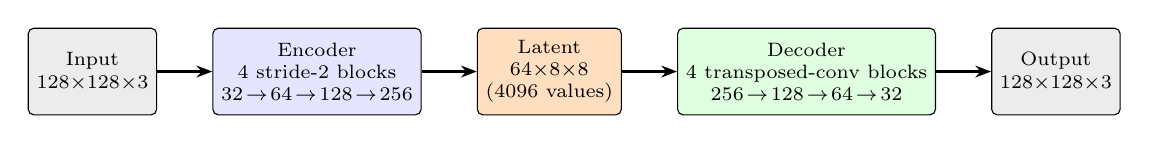
\begin{tikzpicture}[
  node distance=5mm and 7mm,
  blk/.style={draw, rounded corners=2pt, align=center, font=\scriptsize, minimum height=11mm, inner sep=3pt},
  io/.style={blk, fill=gray!15},
  enc/.style={blk, fill=blue!10},
  lat/.style={blk, fill=orange!25},
  dec/.style={blk, fill=green!12},
  arr/.style={-{Stealth[length=2mm]}, thick}]
  \node[io] (in) {Input\\$128{\times}128{\times}3$};
  \node[enc, right=of in] (e) {Encoder\\4 stride-2 blocks\\$32\!\to\!64\!\to\!128\!\to\!256$};
  \node[lat, right=of e] (z) {Latent\\$64{\times}8{\times}8$\\(4096 values)};
  \node[dec, right=of z] (d) {Decoder\\4 transposed-conv blocks\\$256\!\to\!128\!\to\!64\!\to\!32$};
  \node[io, right=of d] (out) {Output\\$128{\times}128{\times}3$};
  \draw[arr] (in)--(e); \draw[arr] (e)--(z); \draw[arr] (z)--(d); \draw[arr] (d)--(out);
\end{tikzpicture}
\caption{Task 1 universal autoencoder (final model, no skip connections). The same backbone with a narrow skip option was used in the ablation.}\label{fig:ae}
\end{figure*}

\subsection{Loss and training}
With clean image $x$ and reconstruction $\hat{x}$ the loss is
\begin{equation}
\mathcal{L}=\alpha\,\lone(x,\hat{x})+(1-\alpha)\bigl(1-\ssim(x,\hat{x})\bigr).
\end{equation}
The $L_1$ term drives accurate pixel values and the SSIM term preserves structure. The final model was trained for 100 epochs with batch size 32, learning rate $4.55\times10^{-4}$, dropout 0.1 and $\alpha=0.6$ (selected by Optuna).

\subsection{Hyperparameter search and design history}
The design evolved over three Optuna studies, each motivated by the previous result (Table~\ref{tab:t1hist}). \textbf{v1} used a flattened linear bottleneck (up to 512 values). Its test PSNR was nearly flat across inputs (about 17.4--18.1\,dB, even for clean images), indicating that the vector bottleneck, not training length, limited quality: 60 epochs gave only 0.447 against 0.395 for an 8-epoch trial. \textbf{v2} replaced the vector by a spatial $8{\times}8$ latent that keeps the image layout. \textbf{v3} added a narrow skip connection to the search space (width 0, 2, 4 or 8) to test whether limited skips help.

\begin{table*}[t]
\centering
\caption{Design history of the universal autoencoder. Optuna: trials (completed/pruned) $\times$ epochs per trial. Test metrics are overall means over 36{,}690 test conditions.}\label{tab:t1hist}
\footnotesize\setlength{\tabcolsep}{4pt}
\begin{tabular}{@{}llcccc@{}}
\toprule
Version & Bottleneck & Optuna & Final epochs & Val.\ score & Test PSNR / SSIM\\
\midrule
v1 & flat vector (512) & 20 (8/12) $\times$ 8 & 60 & 0.447 & 17.85 / 0.439\\
v2 & spatial $8{\times}8{\times}32$ & 20 (8/12) $\times$ 8 & 40 & 0.584 & 20.52 / 0.639\\
v3, skip 4 & spatial $8{\times}8{\times}64$ + narrow skip & 24 (9/15) $\times$ 12 & 100 & 0.639 & not evaluated\\
\textbf{v3, no skip (final)} & spatial $8{\times}8{\times}64$ & (same study) & 100 & \textbf{0.646} & \textbf{21.63 / 0.735}\\
\bottomrule
\end{tabular}
\end{table*}

The v3 search space was: learning rate $[5{\times}10^{-5},3{\times}10^{-3}]$ (log), batch size $\{16,32,64\}$, latent channels $\{16,32,48,64\}$, base channels $\{32,48,64\}$, dropout $[0,0.3]$, $\alpha\in[0.5,0.95]$ and skip width $\{0,2,4,8\}$. Of 24 trials, 9 completed and 15 were pruned; the best trial (objective 0.6028 after 12 epochs) used latent 64, base 32, $\alpha=0.6$ and skip width 4. The earlier studies searched a flat bottleneck in $\{64,128,256,512\}$ (v1) and latent channels $\{4,8,16,32\}$ (v2). Figure~\ref{fig:t1optuna} shows the optimisation history and parameter importances of the v3 study.

\begin{figure}[t]
\centering
\safegraphic[width=0.49\linewidth]{optuna/task1_ae_v3_history.png}\hfill
\safegraphic[width=0.49\linewidth]{optuna/task1_ae_v3_importance.png}
\caption{Task 1 (v3) Optuna study: optimisation history (left) and parameter importance (right).}\label{fig:t1optuna}
\end{figure}

\subsection{Are skip connections needed? A controlled ablation}
The assignment permits limited skips if investigated. In 15-epoch runs with otherwise identical settings, a narrow skip helped (Table~\ref{tab:abl}): width 4 and 8 reached 0.606 and 0.610 against 0.575 and 0.569 without a skip, and widening the latent alone (64 vs.\ 32 channels) did not help. However, short runs favour skips, which speed up early learning. We therefore trained the Optuna-best configuration for 100 epochs with and without the skip: the no-skip model scored \textbf{0.646} (SSIM 0.745, PSNR 21.88\,dB) and the skip model 0.639 (SSIM 0.734, PSNR 21.75\,dB). The gap is small and based on one seed each, so we do not claim the skip hurts, only that it gives no benefit at convergence. We chose the \textbf{no-skip model} as the final Task 1 model: it is at least as accurate, simpler, and satisfies the bottleneck requirement without needing justification. Skip width 4 adds 1{,}024 values (a $16{\times}16{\times}4$ map), well below the 4{,}096-value latent.

\begin{table}[t]
\centering
\caption{15-epoch ablation of latent width and narrow skip (validation score $J$; one seed per row).}\label{tab:abl}
\footnotesize\setlength{\tabcolsep}{4pt}
\begin{tabular}{@{}lcccc@{}}
\toprule
Run & A & B & C & D\\
\midrule
Latent channels & 32 & 64 & 32 & 32\\
Skip width & 0 & 0 & 4 & 8\\
Validation score $J$ & 0.575 & 0.569 & 0.606 & 0.610\\
\bottomrule
\end{tabular}
\end{table}

\begin{figure}[t]
\centering
\safegraphic[width=\linewidth]{curves/task1_val_score.png}
\caption{Task 1 final training: validation score versus epoch for the skip and no-skip runs. \todo{export from W\&B and save as report\_figures/curves/task1\_val\_score.png}}\label{fig:t1curve}
\end{figure}

\subsection{Results}
Table~\ref{tab:t1res} reports the final model on the official test set, separately per condition and severity, next to the unrestored input. Qualitative results appear in Fig.~\ref{fig:t1ex1}--\ref{fig:t1ex2} (12 examples: clean target, corrupted input, reconstruction and absolute-error map) and Fig.~\ref{fig:t1fail}.

\begin{table}[t]
\centering
\caption{Task 1 test results (final no-skip model) versus the unrestored input.}\label{tab:t1res}
\footnotesize\setlength{\tabcolsep}{3pt}
\begin{tabular}{@{}lrrrrr@{}}
\toprule
Condition & $n$ & PSNR$_{in}$ & PSNR$_{out}$ & SSIM$_{in}$ & SSIM$_{out}$\\
\midrule
Overall & 36690 & 22.34 & 21.63 & 0.671 & 0.735 \\
\midrule
Clean & 3669 & 50.00 & 22.45 & 1.000 & 0.775 \\
\midrule
Salt-and-pepper & 11007 & 16.38 & 22.34 & 0.382 & 0.760 \\
\quad Low & 3669 & 20.14 & 22.44 & 0.603 & 0.771 \\
\quad Medium & 3669 & 15.87 & 22.37 & 0.339 & 0.762 \\
\quad High & 3669 & 13.14 & 22.20 & 0.204 & 0.745 \\
\midrule
Gaussian blur & 11007 & 27.82 & 22.33 & 0.814 & 0.753 \\
\quad Low & 3669 & 32.34 & 22.54 & 0.944 & 0.774 \\
\quad Medium & 3669 & 26.77 & 22.49 & 0.806 & 0.765 \\
\quad High & 3669 & 24.35 & 21.97 & 0.692 & 0.721 \\
\midrule
Occlusion & 11007 & 13.59 & 19.96 & 0.709 & 0.678 \\
\quad Low & 3669 & 16.68 & 21.11 & 0.862 & 0.730 \\
\quad Medium & 3669 & 13.34 & 20.05 & 0.727 & 0.686 \\
\quad High & 3669 & 10.74 & 18.72 & 0.538 & 0.619 \\
\bottomrule
\end{tabular}
\end{table}

\textbf{Interpretation.} The universal model clearly helps for salt-and-pepper noise (SSIM 0.382$\to$0.760 and PSNR 16.4$\to$22.3\,dB, with 0.204$\to$0.745 SSIM at the highest severity). Its output quality is almost independent of the input: about 22.2--22.5\,dB for clean inputs and for all three noise severities. This is the signature of a capacity ceiling set by the bottleneck, not of condition-specific restoration. The cost is visible on inputs that need no restoration: clean images drop to 22.45\,dB and mild blur drops from 32.34 to 22.54\,dB, so for Gaussian blur the output is below the input in both PSNR and SSIM at every severity. Occlusion is the only condition where output quality depends on severity (PSNR 21.11\,dB at low severity versus 18.72\,dB at high); PSNR improves over the input (13.59$\to$19.96\,dB), but overall SSIM is lower (0.709$\to$0.678) because unaffected regions are blurred. Compared with the design history (Table~\ref{tab:t1hist}), moving from the vector to the spatial latent raised test SSIM from 0.439 to 0.639, and the final model reached 0.735. These limits motivate Tasks 2 and 3, where clean inputs bypass restoration.

\begin{figure*}[t]
\centering
\safegraphic[width=0.78\textwidth]{task1/examples_1.png}
\caption{Task 1 examples (1/2): rows show clean target, corrupted input, reconstruction and absolute error (test set, fixed manifest).}\label{fig:t1ex1}
\end{figure*}
\begin{figure*}[t]
\centering
\safegraphic[width=0.78\textwidth]{task1/examples_2.png}
\caption{Task 1 examples (2/2).}\label{fig:t1ex2}
\end{figure*}

\subsection{Failure cases}
Figure~\ref{fig:t1fail} shows the worst test image per condition.
\begin{enumerate}
\item \textbf{Clean input, PSNR 16.2\,dB, SSIM 0.41.} A dog in a flower field: dense, high-frequency texture cannot be stored in the latent, so the reconstruction loses detail and colour and comes out blurry and sepia-toned.
\item \textbf{Salt-and-pepper (high), SSIM 0.38, and Gaussian blur (high), SSIM 0.35.} The same image is the worst case for the clean, noisy and blurred inputs. The failure is therefore driven by image content (texture), not by the corruption type.
\item \textbf{Occlusion (high), PSNR 11.3\,dB, SSIM 0.26.} A cat on a black background. Black masks are indistinguishable from the background, so the model cannot tell which dark regions are missing content; it fills the hole with a grey haze that spills into the empty background, and the error map is brightest there.
\end{enumerate}

\begin{figure}[t]
\centering
\safegraphic[width=\linewidth]{task1/failure_cases.png}
\caption{Task 1 failure cases (worst SSIM per condition): clean, salt-and-pepper (high), blur (high), occlusion (high).}\label{fig:t1fail}
\end{figure}

\subsection{ONNX export and application}
The final model is exported to ONNX (10.2\,MB; maximum absolute output difference to PyTorch $1.06\times10^{-6}$; 18\,ms per image on CPU, Section~\ref{sec:onnx}) and available in the application under \emph{Universal Restoration}.

% ===== END OF PART 1 =====